\documentclass{article}
\title{Notes for: Algorithms for Inverse Reinforcement Learning}
\author{-- \thanks{paper: https://ai.stanford.edu/~ang/papers/icml00-irl.pdf}}
\date{\today}
\usepackage{graphicx}

\begin{document}
    \maketitle
    
    \section{High Level and Motivation}

    \subsection{Problem}
    
    \begin{itemize}
        \item Normal reinforcement learning is the process of extracting an optimal policy for a given reward function in an environment.
        \item Inverse reinforcement learning is the process of extracting a reward function from an environment given observed \textbf{optimal behavior}.
    \end{itemize}
    
    \subsection{Example}
    You are able to observe an agent's actions as it tackles a modified version of the Mountain Car problem:


    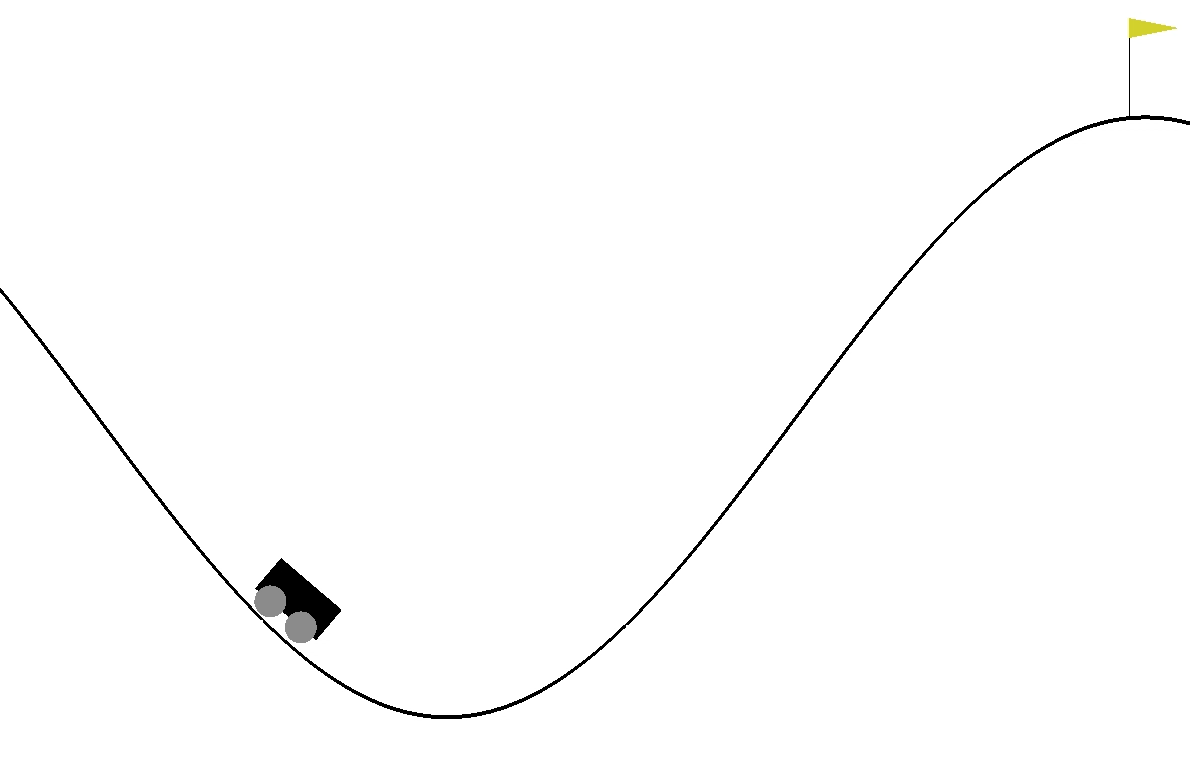
\includegraphics[width=7cm]{fig1.png}


    In the normal case, the car's aim is to reach the yellow flag where it will receive a reward.

    In the modified case, which interests us, the car driving agent was trained to reach a different location (unknown to us) by being provided a different reward signal. 

    We have access to:

    \begin{enumerate}
        \item the examples of the driving agent's actions over time
        \item the state before each decision was made, and
        \item a model of the environment
    \end{enumerate}

    Our goal is to uncover what the reward signal is.

    A key issue not addressed by the paper is the fact that the agent may not exhibit \textbf{optimal behavior} for that reward signal.

    


    \section{Medium Level}

    \section{Low Level}

\end{document}